\documentclass[a4paper,fleqn,usenatbib]{mnras}
\usepackage{newtxtext,newtxmath}
\usepackage[T1]{fontenc}
\usepackage{ae,aecompl}
\usepackage{graphicx}
\usepackage{amsmath}
\usepackage{amssymb}
\usepackage{nccmath}
\usepackage[utf8]{inputenc}
\newcommand{\fhat}[1]{\expandafter\hat#1}
\newcommand{\fbar}[1]{\expandafter\bar#1}
\newcommand\fnurl[2]{%
  \href{#2}{#1}\footnote{\url{#2}}%
}

\title[Splashback radius in Pan-STARRS / Planck-SZ data]{Detection of the Splashback Radius by Cross-Correlation of Pan-STARRS and Planck-SZ data}

\author[D. Zürcher]{
D. Zürcher,$^{1}$\thanks{E-mail: dominikz@student.ethz.ch}
Supervisor: S. More,$^{2}$
Co-Supervisor: A. Refregier $^{3}$
\\
$^{1}$Department of Chemistry and Applied Biosciences, ETH Zurich, Vladimir-Prelog-Weg 1, 8093 Zurich, Switzerland\\
$^{2}$Kavli Institute for the Physics and Mathematics of the Universe (Kavli IPMU, WPI), \\ The University
of Tokyo, 5-1-5 Kashiwanoha, Kashiwa, Chiba 277-8583\\
$^{3}$Department of Physics, ETH Zurich, Wolfgang Pauli Strasse 27, 8093 Zurich, Switzerland\\
\\
Master's Thesis\\
In partial fulfillment of the requirements for the Master of Science ETH in Interdisciplinary Sciences 
}

% These dates will be filled out by the publisher
%\date{Accepted XXX. Received YYY; in original form ZZZ}

\pubyear{2018}

\begin{document}
\label{firstpage}
\pagerange{\pageref{firstpage}--\pageref{lastpage}}
\maketitle

% Abstract of the paper
\begin{abstract}
This is a simple template for authors to write new MNRAS papers.
The abstract should briefly describe the aims, methods, and main results of the paper.
It should be a single paragraph not more than 250 words (200 words for Letters).
No references should appear in the abstract.
\end{abstract}

\begin{keywords}
galaxies:clusters:general -- galaxies:halos -- methods:observational -- cosmology:dark matter -- cosmology:large-scale structure of Universe -- cosmology:observations
\end{keywords}

\section{Introduction}
Being one of the major and most promising probes in modern cosmology, the understanding of structure formation is getting a lot of attention from the observational, as well as from the theoretical side. In the standard framework of structure formation galaxies form via dissipative processes of baryons falling into the gravitational potential wells of dark matter clumps, so called halos\citep{rees1977cooling,white1978core,fall1980formation,blumenthal1984formation}. To infer constrains on the cosmological parameters from observations of the large scale galaxy distribution a profound understanding of the processes converting baryons into stars, as well as the growth rates of the halos is needed. Especially the scaling relation between the luminosity of galaxies and the dark matter halos associated with them have to be known in order to understand the process of structure formation \citep{kravtsov2004dark}. While the understanding of the scaling relation requires both; knowledge of the production of stars in the halos as well as the growth rate of the halos themselves, we only focus on the later in this work.

\citet{diemer2014dependence} studied the outskirts of the mass profiles of dark matter halos, which received only little attention in past studies compared to the inner regions of the halos. They showed, that classical fitting functions such as the Navarro-Frenk-White or the Einasto profile fail to describe the outer parts of the mass profiles as inferred from N-body simulations. Particularly they found a sharp steepening of the profile around the virial radius $r \approx R_{\mathrm{200m}}$, which is not modeled correctly by those fitting functions. They proposed a new fitting function consisting of an inner Einasto profile and an outer power law profile connected by a smooth transition
\begin{align}
\rho(r)=\rho_{\mathrm{in}}(r)f_{\mathrm{trans}}(r) + \rho_{\mathrm{out}}(r) 
\label{eq:model} \\
\rho_{\mathrm{in}}(r)=\rho_s\exp\left( -\frac{2}{\alpha}\left[ \left( \frac{r}{r_s}\right)^{\alpha}-1 \right] \right) \\
f_{\mathrm{trans}}(r)=\left( 1+\left( \frac{r}{r_t} \right)^{\beta} \right)^{-\gamma/ \beta} \\
\rho_{\mathrm{out}}(r)=\rho_0\left( \frac{r}{r_{out}}\right)^{-s_e}
\end{align}
where $r$ indicates the three dimensional radial distance from the halo center \citep{diemer2014dependence}.

In a follow up study \citet{adhikari2014splashback} proposed a simple theoretical model, which is able to accurately reproduce the sharp steepening found by Diemer and Kravtsov before. They argued that caustics arise in triaxial collapses of dark matter due to a pile up of the orbits of multiple particles at a similar radius. Such caustics most frequently appear close to the apocenters of the orbits due to the radial velocity being very small at that point, which causes the particles to spend a longer time there \citep{lithwick2011self}. The outermost caustic of a halo is associated with the first apoapsis of the most recently accreted particles. Those particles underwent a first collapse meaning that they passed through the center of the halo just once. This phenomenon is termed splashback effect and the radius corresponding to the density drop after the outermost caustic has been named splashback radius correspondingly. The location of the splashback radius depends mainly on the accretion rate $\Gamma$ of the halo, but shows a small redshift dependence due to the influence of $\Omega_{\mathrm{m}}$ . At lower redshifts $\Omega_{\mathrm{m}}$ decreases quickly leading to a smaller matter background density, which causes the halo to accrete less matter per time. Therefore the potential well deepens less quickly while the particles are traveling on their orbits and the splashback radius shifts towards larger radii. On the other hand, a higher accretion rate leads to a quicker deepening of the potential well of the halo, causing the splashback radius to occur at smaller radii. Therefore, the location of the splashback radius can be used to infer the accretion rate of a halo \citep{adhikari2014splashback}.

Motivated by the collapse model of a spherical top-hat over-density the outer boundary of a halo is usually defined as a radius $R_\Delta$ enclosing a region with an over-density of $\Delta$ or more with respect to a certain reference density $\Delta_{\mathrm{ref}}$, where the lower bound of the required over-density is given from the virialization criterion \citep{gunn1972infall}. However, \citet{diemer2013pseudo} found that such a boundary definition can lead to pseudo-evolution of the halo mass, meaning an apparent growth of the halo mass that is caused only by the evolution of the reference density with redshift and not by a physical accretion of mass onto the halo. Using simulations they showed that pseudo evolution accounts for nearly all of the apparent growth between $z=1$ and $0$ of galaxy-sized halos and can also account for a substantial fraction of the growth of cluster-sized halos \citep{diemer2013pseudo}. Further, \citet{diemer2013pseudo} realized that a new definition for the boundary of halos is required which must not suffer from pseudo-evolution. \citet{more2015splashback} proposed to use the newly discovered splashback radius as such an alternative definition. They found that depending on the accretion rate of the halo, the splashback radius may lay well beyond the commonly used virial radius. For slowly accreting halos the splashback radius is expected to occur at $\approx 0.8-1$ $R_{\mathrm{200m}}$ and at $\approx 1.5$ $R_{\mathrm{200m}}$ for quickly accreting halos \citep{more2015splashback}.

Using data from the Sloan Digital Sky Survey (SDSS) Data Release 8 (DR8) photometric galaxy catalog \citet{more2016detection} were able to confirm the existence of the splashback radius in observations. \citet{more2016detection} used galaxy clusters identified from the SDSS DR8 catalog by the redMaPPer algorithm \citep{rykoff2014redmapper,rozo2015redmapper}. The galaxy clusters were divided into two subsamples with the same redshift and mass distributions but different internal distributions of the galaxies within the halos. The same division has already been used by \citet{miyatake2016evidence} before and the samples have been shown to have different large-scale clustering amplitudes. By studying the stacked surface density profiles of the galaxy clusters \citet{more2016detection} detect a sharp steepening in both subsamples providing strong evidence for the existence of the splashback effect. Due to the splashback radius appearing at different locations in the two subsamples it was concluded that the two samples inherit different accretion rates implying different assembly histories. Therefore, halo assembly bias has been detected meaning that the clusters differ in their large scale distribution while having the same masses but different assembly histories \citep{more2016detection}. 

\citet{more2016detection} compared their findings with simulations by utilizing the MultiDark-Planck II N-body simulation \citep{klypin2016multidark}. The comparison showed that the splashback radii detected for both subsamples are too small and also that the detected halo assembly bias signal is larger than expected from the simulation. Using the same N-body simulation once more \citet{more2016detection} explored several systematic effects which could lead to such deviations. However, none of the investigated, systematic effects can account for the discrepancies found in the data. However, \citet{more2016detection} noted that they cannot completely rule out the influence of effects originating from weak lensing as well as projections and optical cluster finding: The weak lensing signal is used in order to infer the masses $M_{\mathrm{200m}}$ and radii $R_{\mathrm{200m}}$ of the clusters. However, miscalibrations of the observable halo mass relations by weak lensing cannot be ruled out with today's data. In addition the weak lensing mass estimate is based solely on the projected mass distribution of the cluster. Therefore, different clusters might have different three-dimensional mass distributions although they possess the same weak lensing signal. Further, the identification of the central galaxy in a cluster is performed by the redMaPPer algorithm. This process of optical cluster finding is known to be affected by mis-centering. Mis-centering refers to the algorithm picking the wrong galaxy to be the central galaxy, or to the displacement of the central galaxy from the potential minimum of the cluster. Ruling out the influence of those systematic effects, with the discrepancy in the position of the splashback radius still remaining, would clear the path for new physical insights: Firstly, such a finding might point towards higher accretion rates of matter onto halos than expected from the standard cosmological model so far \citep{adhikari2016observing}. Alternatively, the introduction of anisotropic dark matter self-interactions into the dark matter model could account for the discrepancy while still obeying the bounds imposed by sub-halo evaporation \citep{kahlhoefer2013colliding}. Both explanations impose interesting challenges for the standard cosmological model and may point towards new physics\citep{more2016detection}.

In this work the influence of the effects mentioned above is removed by using an independent catalog of galaxy clusters, namely the second Planck Catalogue of Sunyaev-Zeldovich Sources (PSZ2), which is part of the 2015 data release of the Planck mission. The used catalog consists out of 1653 clusters detected by the Planck satellite  \citep{collaboration2016planck} by the use of the Sunyaev-Zeldovich effect. The estimate of the positions as well as the cluster masses are not affected by the effects mentioned above. As for the galaxies, the $3\upi$ Steradian survey, which is part of the Panoramic Survey Telescope and Rapid Response System (Pan-STARRS) Data Release 1 (DR1) is utilized \citep{chambers2016pan}. A similar analysis as in \citep{more2016detection} is carried out and new methods are being explored.

This paper is organized as follows: Section 2 starts by introducing the data, namely the cluster and the galaxy catalog as well as the methods that are used to derive the results which are presented in visual and tabular form and shortly discussed in Section 3. The results and their implications are discussed in great detail in Section 4 and finally we summarize our findings in Section 5 and provide a short outlook on what has yet to be done.

\section{Data and Methods}
In order to carry out the analysis described by \citet{more2016detection} two datasets are required. Firstly, a cluster catalog is needed. In \citet{more2016detection} this catalog is obtained from the SDSS DR8 sample using the RedMaPPer cluster finding algorithm. Here it is substituted by the larger PSZ2 catalog, which does not suffer from the systematic effects mentioned in the last section. On the other hand, the galaxy catalog, being the SDSS DR8 catalog in \citet{more2016detection}, is replaced by the larger and deeper Pan-STARRS DR1 catalog. In this section the used catalogs are described and the methods that are exploit are introduced.

\subsection{Cluster catalog}
\label{sec:clusters}
The dominant, baryonic component of a galaxy cluster is the hot, ionized  intra-cluster medium (ICM) which is trapped within the cluster. Via inverse Compton scattering the ICM can increase the energy of photons originating from the cosmic microwave background (CMB) that pass through the cluster. This effect is known as the thermal Sunyaev-Zeldovich (SZ) effect \citep{sunyaev1970small,sunyaev1980velocity}. The imprint of the effect on the CMB is best visible in the X-Ray range above 220 GHz. The High Frequency Instrument (HFI) of the Planck satellite is suited perfectly to observe the sky at this frequency \citep{collaboration2016planck}. Having, imaged the whole sky with an angular resolution and frequency coverage that was never achieved by any previous mission, the Planck satellite launched on May 14th 2009 was able to produce the largest SZ-selected sample of galaxy clusters yet. Being part of the 2015 Data Release of the Planck mission the second Planck Catalogue of Sunyaev-Zeldovich Sources (PSZ2) counts 1653 galaxy cluster detections, of which 1203 have been confirmed by cross-matching with other galaxy clusters from external data sets. The 67\% error radius of the cluster positions is $1.5\arcmin$ and the estimated purity of the catalog has a lower limit of 83\% (probability that a detection corresponds to a real object) \citep{adam2016planck,collaboration2016planck}. The PSZ2 catalog is publicly available from the \fnurl{\textit{Planck Legacy Archive}}{https://pla.esac.esa.int/pla/\# home}. 

From the 1653 objects in the catalog only those with a redshift $0.03 \leq z \geq 0.33$ are chosen in order to reproduce the same conditions as in \citet{more2016detection}. As discussed extensively in \citet{more2016detection} already, galaxy cluster positions are often affected by misplacement. To avoid biases caused by such misplacements, images from the Pan-STARRS DR1 survey centered at the galaxy cluster positions are inspected visually. Assuming that the center of the cluster coincides with the position of the brightest cluster galaxy (BCG) the positions are adjusted manually. The final sample then consists out of 596 galaxy clusters which is small compared to a sample size of 8643 clusters as used by \citet{more2016detection}. The average redshift of the sample lies at 0.177 and the median at 0.179 whereas the average cluster mass amounts to $4.335 \cdot 10^{14} $M$_{\sun}$ with a median of $4.143 \cdot 10^{14} $M$_{\sun}$. Table~\ref{tab:cluster_catalogs} shows a comparison of the major properties of the two different cluster catalogs as used in this work and in \citet{more2016detection}. See Figure~\ref{fig:planck_fig} in Appendix~\ref{sec:figures} for a HEALPix map showing the cluster positions as well as the survey selection function \citep{2005ApJ...622..759G}.

Assuming the presence of a foreground and background population of clusters in the data a random cluster catalog is required to remove the effects of such a contamination (see Section~\ref{sec:estimators}). Exploiting the selection function of the PSZ2 survey which is also publicly available on the \fnurl{\textit{Planck Legacy Archive}}{https://pla.esac.esa.int/pla/\# home} a random galaxy sample composed of 8470 objects is constructed. The redshifts of the objects are drawn randomly from the redshifts of the actual cluster catalog in order to reproduce the same redshift distribution.


\begin{table}
    \centering
    \caption{Comparison of the PSZ2 cluster catalog against the RedMaPPer catalog used by \citet{more2016detection}. The values of the mass estimates $M_{\mathrm{500c}}$, $M_{\mathrm{200m}}$, redshifts $z$ and expected splashback radii $r^{\mathrm{3D,theo}}_{\mathrm{sp}}$ represent the catalog averages. The conversions of the masses as well as the calculation of the expected splashback radii was performed using the Python package COLOSSUS \citep{diemer2017colossus}.}
    \label{tab:cluster_catalogs} 
    \begin{tabular}{|c|c|c|c|}
    \hline 
    & RedMaPPer & PSZ2 & MCXC \\ 
    \hline 
    $z$ & 0.24 & 0.177 & \\ 
    \hline 
    \# objects & 8643 & 596 & \\ 
    \hline
    $M_{\mathrm{500c}}$ [$10^{14} $M$_{\sun}$] & 1.0 & 4.3 & \\ 
    \hline
    $M_{\mathrm{200m}}$ [$10^{14} $M$_{\sun}$] & 1.8 & 8.6 & \\ 
    \hline
    $r^{\mathrm{3D,theo}}_{\mathrm{sp}}$ [h$^{-1}$ Mpc] & 1.10 & 1.73 & \\ 
    \hline
    \end{tabular} 
\end{table}

\subsection{Galaxy catalog}
\label{sec:galaxies}
The Panoramic Survey Telescope and Rapid Response System (Pan-STARRS) is a wide-field astronomical imaging and data processing facility operated by the University of Hawaii's Institute for Astronomy \citep{kaiser2002pan,kaiser2010pan}. The data for the Data Release 1 (DR1) was gathered using a single 1.8 meter dish telescope equipped with a 1.4 gigapixel camera, which is located on Maui. We use the 3$\upi$ Steradian Survey which is part of the DR1. The survey covers the sky north of $\delta=-31\degr$ (ICRS) in five broadband filters ($g_{\mathrm{P1}}, r_{\mathrm{P1}}, i_{\mathrm{P1}}, z_{\mathrm{P1}}, y_{\mathrm{P1}}$). In order to obtain deeper images the survey stacks pictures taken from 2009-06-02 until 2014-03-31. The achieved, band-dependent depth amounts to (23.3, 23.2, 23.1, 22.3, 21.4) magnitudes for the individual bands, respectively. Further, the magnitude of the objects is determined up to a standard deviation of 7-12 mmag depending on the band and the position of the objects is measured with a standard deviation of $\Delta ra=2.3\arcsec$ and $\Delta \delta=1.7\arcsec$. The Pan-STARRS survey uses a modification of the Budavari rings tessellation pattern to organize the data. The sky is split into rings with their middles spaced $4 \degr$ apart in declination space. Each ring is then divided into \textit{projectioncells} where the number of \textit{projectioncells} in each ring varies with declination. Notice that the \textit{projectioncells} overlap at some points. Having a size of roughly $4\degr$x$4\degr$, the \textit{projectioncells} are very large and inconvenient for the end user to handle. Therefore, they are further subdivided into 10x10 \textit{skycells}, each with a size of roughly $0.4\degr$x$0.4\degr$ which overlap by $60\arcsec$ (120 pixels) on each side in order to prevent splitting of objects. The survey has a global pixel scale of $0.25\arcsec$ \citep{chambers2016pan}. 

The 3$\upi$ Steradian Survey consists out of multiple data products and not all of them are used in this work. Image-wise, we use the polychromatic \textit{stack} images to perform the visual correction of the cluster center locations and the \textit{stack.mask} images to disregard objects laying in bad pixel regions. Data-wise, we extract the galaxy catalog from the \textit{StackObjectThin} table. The data table is publicly available on the \fnurl{\textit{Barbara A. Mikulski Archive for Space Telescopes} (MAST)}{http://archive.stsci.edu/}. We select only objects with the \textit{BestDetection} flag attached to them indicating that they have been detected with acceptable accuracy. Due to the splitting of the survey in \textit{projectioncells} and \textit{skycells} and the induced overlapping of the cells, objects may show up in multiple cells and are therefore listed multiple times in the data table. Therefore, we keep only objects with the \textit{PrimaryDetection} flag attached which avoids counting the same object multiple times. 

The magnitudes of the selected objects are then corrected for the extinction caused by the dust present in the Milky Way. This is done using the \fnurl{mwdust}{https://github.com/jobovy/mwdust} Python module provided by \citet{bovy2016galactic}. The extinction correction is performed using a dust map combining the measurements of \citet{marshall2006modelling}, \citet{green2015three} and \citet{drimmel2003three}. Only objects with an extinction corrected magnitude up to 22.0 as measured in the $i_{P1}$ band are selected from the catalog. After this procedure, the extracted galaxy counts exactly 1'155'285'728 objects. Starting from this catalog three different sub-catalogs named PS 21, PS 21.5 and PS 22 with a survey depth of 21.0, 21.5 and 22.0 magnitude, respectively are constructed.

As mentioned in the description of the Pan-STARRS survey by \citet{chambers2016pan} there is a significant variation in the depth of the 3$\upi$ Steradian survey even on small scales. In order to avoid choosing objects in shallow regions of the survey the minimal observed Kron magnitude in the $i_{\mathrm{P1}}$ band in each \textit{skycell} is recorded and only objects in skycells with a minimal observed Kron magnitude of 21.0, 21.5 and 22.0 or higher are selected depending on the corresponding catalog. Since most of the shallow regions lay in the galactic plane the whole region with $-20.0 < b < 20.0$ in galactic coordinates is excluded on top of that. The HEALPix maps showing the excluded areas on the sky are included in Appendix~\ref{sec:heal_maps}. To disregard objects laying in bad pixel regions caused for example by nearby, bright stars or camera artifacts a masking procedure is performed using the \textit{stack.mask} objects.

Since the Pan-STARRS survey contains galaxies and stars alike a star-galaxy separation has to be applied. Therefore, a simple cut in the PSF - Kron magnitude space in the $i_{\mathrm{P1}}$ band is used. All objects with a value of $i_{\mathrm{P1,PSF}} - i_{\mathrm{P1,Kron}}> 0.05$ are considered to be galaxies and all other objects are disregarded. As pointed out by \citet{farrow2013pan} this separation does a fairly good job. Bright, close-by stars tend to be classified as extended objects, therefore stars are often classified as galaxies by such a selection at magnitudes below 13.5 \citep{chambers2016pan}. To avoid contamination of the data with bright stars all objects with a $i_{\mathrm{P1,PSF}} < 15.0$ are disregarded. Since there are basically no galaxies at such low magnitudes this does not introduce a selection bias. In Table~\ref{tab:galaxy_catalogs} the major properties of the extracted galaxy catalogs are summarized and compared to the SDSS catalog as used in \citet{more2016detection}. 

%(describe properties / expectations)
%Catalogs are publicly available???

Since it has to be assumed that there is a contamination by foreground and background galaxies present a random galaxy catalog is required (see Section~\ref{sec:estimators}). The random catalog is created by uniformly generating objects on the unit sphere and disregarding all objects laying in those regions that have been excluded in the galaxy catalog as well. Therefore, for each galaxy catalog a corresponding random catalog is generated.

\begin{table*}
    \centering
    \caption{Summary and comparison of the properties of the galaxy catalogs used in this work as well as the SDSS catalog used in \citet{more2016detection}.}
    \label{tab:galaxy_catalogs}
    \begin{tabular}{|c|c|c|c|c|}
    \hline 
    & SDSS & PS 21 & PS 21.5 & PS 22 \\ 
    \hline 
    depth [mag] & 21.43 & 21.00 & 21.50 & 22.00\\ 
    \hline 
    eff. area [deg$^2$] & $\approx$ 10'000 & 19'515 & 20'586 & 15'689\\ 
    \hline 
    \# objects & 57'181'113 & 87'985'151 & 123'188'529 & 105'809'113 \\
    \hline
    objects/deg$^2$ & 5718 & 4509 & 5984 & 6744\\ 
    \hline
    \end{tabular} 
\end{table*}


\subsection{Estimation of the spatial density profile}
\label{sec:estimators}
The splashback radius manifests itself as a sharp steepening in the spatial density profile of a dark matter halo. Unfortunately, such profiles are not directly accessible by todays measurements. However, in the standard paradigm of structure formation it is assumed that galaxies track the underlying dark matter distribution since they form from baryonic matter falling into the potential wells created by the dark matter \citep{rees1977cooling,white1978core,fall1980formation,blumenthal1984formation}. Therefore, I shall use the radial galaxy distribution as a proxy for the dark matter distribution of a halo. A further complication arises by the fact that only the projected galaxy distribution within a halo is accessible as a projection of the three dimensional distribution onto a projection plane perpendicular to the line of sight. Therefore, the three dimensional model given in Equation~\ref{eq:model} needs to be integrated along the line of sight in order to obtain a model for the surface density profile:
\begin{equation}
\xi(R)=2\int^{x_{max}}_0 \rho(\sqrt{R^2+x^2}) dx 
\label{eq:surface}
\end{equation}
where we adopt $x_{\mathrm{max}}=40 $ h$^{-1}$Mpc for the maximum projection length as suggested by \citet{more2016detection}. The surface density profile $\xi(R)$ depends on the projected radius $R$, which is defined as the projection of the three dimensional, radial distance from the cluster center onto the projection plane.

To obtain a measurement of the surface density profile from the data the cluster catalog is cross-correlated with the galaxy catalog. In order for a galaxy to be associated with a certain cluster the projected radial distance from the cluster center position must be  $\leq$ 10 h$^{-1}$ Mpc. Notice that since the clusters in the catalog span a large redshift range there will be a selection bias originating from systematically detecting more faint galaxies in low redshift clusters. To avoid such systematics a galaxy's magnitude m$_{\mathrm{gal}}$ must fulfill the following constraint to be considered as being part of a cluster at redshift z$_{\mathrm{clu}}$:
\begin{equation}
m_{\mathrm{gal}} < m_{\mathrm{lim}} - 5 \log_{10} \left( \frac{D(z_{\mathrm{clu}})}{D(z_{\mathrm{max}})} \frac{1+z_{\mathrm{max}}}{1+z_{\mathrm{clu}}}  \right)
\label{eq:constraint}
\end{equation}
where the function $D(z)$ determines the comoving distance to an object at redshift $z$. Further $z_{\mathrm{max}}$ is the maximal redshift of the cluster catalog (0.33 in our case) and $m_{\mathrm{lim}}$ indicates the depth of the galaxy catalog in consideration in magnitudes (being 21.0, 21.5 and 22.0, respectively) \citep{more2016detection}.
The assignment of the galaxies to the clusters requires to perform a range search which is done using the Python module \fnurl{splashpipe}{https://github.com/surhudm/splashpipe} which exploits a k-d tree algorithm to do so . The assigned galaxies are then binned into 8 equally spaced radial bins ranging from 0.1 h$^{-1}$ Mpc to 10 h$^{-1}$ Mpc.  

We expect a correlation between clusters and galaxies if they are at the same redshift. However, at the same time it has to be assumed that there will also be a population of uncorrelated galaxies present consisting of higher or lower redshift galaxies that are not associated with the cluster in question. The same holds true for the cluster population as well. Such contaminations can be estimated by the use of random catalogs modeling the uncorrelated component of the two-point cross-correlation function. Following the discussion outlined in \citet{kerscher2000comparison} We shall introduce how the two-point correlation function can be estimated taking into consideration the contaminations mentioned above.


Let us define a counting function $P_{(X,Y)}(D)$, that counts how many objects from the catalog $Y$ can be found at a distance $D$ from any object in catalog $X$ (or vice versa)
\begin{equation}
P_{(X,Y)}(D)=\sum_{x \in X} \sum_{y \in Y} \Phi_D(x,y)
\end{equation}
where 
\begin{equation}
  \Phi_D(x,y) = \left.
  \begin{cases}
    0, & \text{for } d(x,y)<D-\Delta \\
    1, & \text{for }  D-\Delta \leq d(x,y) \leq D+\Delta \\
    0, & \text{for } d(x,y)>D+\Delta
  \end{cases}\right.
\end{equation}
with $d(x,y)$ being the separation between the two objects $x$ and $y$. Since, $X \neq Y$ holds at all times in this work (no auto-correlations of catalogs considered) the normalized counting function can be defined as 
\begin{equation}
P^{\mathrm{N}}_{(X,Y)}(D)=\frac{P_{(X,Y)}(D)}{N_X N_Y}
\end{equation}
with $N_X$ and $N_Y$ being the total number of objects residing in the catalogs $X$ and $Y$, respectively. 
Recalling that we would like to cross-correlate clusters with galaxies we identify one of the catalogs with the cluster catalog (say $X$) and the other one with the galaxy catalog (say $Y$). Further, we note that we are considering the projected, radial separation of objects. Therefore, let us replace the general separation $D$ by the projected, radial distance $R$. For either of the two catalogs we have two choices at hand; namely the actual catalog (further denoted as D) and the corresponding random catalog (further denoted as R) leading to four different counting functions that cross-correlate all the different catalogs; $P^{\mathrm{N}}_{\mathrm{(D,D)}}(R)$,$P^{\mathrm{N}}_{\mathrm{(D,R)}}(R)$,$P^{\mathrm{N}}_{\mathrm{(R,D)}}(R)$,$P^N_{\mathrm{(R,R)}}(R)$.
Starting from those normalized counting functions estimators of the two-point correlation function can be constructed. With the two-point correlation function of galaxies being one of the main statistical tools in cosmology, a vast number of such estimators can be found in the literature. We use the Davis \& Peebles estimator ($\fhat{\xi_{\mathrm{DP}}(r)}$ ; \citep{davis1983survey} ; DP) which corrects only for the contamination stemming from the uncorrelated galaxies and the more sophisticated Landy \& Szalay estimatior ($\fhat{\xi_{\mathrm{LS}}(r)}$ ; \citep{landy1993bias} ; LS) which also exploits the random cluster catalog in order to remove the contamination from back- and foreground clusters as well
\begin{align}
\fhat{\xi_{\mathrm{DP}}(R)}=\frac{P^{\mathrm{N}}_{\mathrm{(D,D)}}(R)}{P^{\mathrm{N}}_{\mathrm{(D,R)}}(R)}-1\\
\fhat{\xi_{\mathrm{LS}}(R)}=\frac{P^{\mathrm{N}}_{\mathrm{(D,D)}}(R)-P^{\mathrm{N}}_{\mathrm{(D,R)}}(R)-P^{\mathrm{N}}_{\mathrm{(R,D)}}(R)+P^{\mathrm{N}}_{\mathrm{(R,R)}}(R)}{P^{\mathrm{N}}_{\mathrm{(R,R)}}(R)}
\end{align}
Hence, we have constructed two estimators for the surface density $\xi(R)$. To estimate the covariance of the calculated surface density profile a jackknife re-sampling approach is taken \citep{efron1982jackknife}. The clusters are subdivided into 21 different jackknife samples. The random clusters are subdivided in the same fashion. In each jackknife bin the redshifts of the random clusters are drawn from the redshifts of the actual clusters in that bin such that the random clusters in each bin inherit the same redshift distribution as their real counterparts. Doing so we construct a set of 30 jackknife estimates for the surface density function
\begin{equation}
\fhat{\xi^{\mathrm{Jack}}_j (R)}=\frac{1}{n-1}\sum^n_{i=1,i\neq j} \fhat{\xi_i (R)}
\end{equation}
where $j \in \{1,..,30\}$ and $n=30$. The $\fhat{\xi_i (R)}$ are the estimates of the surface density function as inferred when considering only the clusters in the jackknife sample $i$. The average $\fbar{\xi(R)}$ and the covariance $\mathrm{Cov}(R_1,R_2)$ of the surface density function are then constructed as
\begin{equation}
\fbar{\xi(R)}=\frac{1}{n}\sum_{j=1}^n \fhat{\xi^{\mathrm{Jack}}_j (R)}
\end{equation}
and 
\begin{equation}
\mathrm{Cov}(R_1,R_2)=\frac{n-1}{n}\sum_{j=1}^n (\fhat{\xi^{\mathrm{Jack}}_j (R_1)} - \fbar{\xi(R_1)}) \cdot (\fhat{\xi^{\mathrm{Jack}}_j (R_2)} - \fbar{\xi(R_2)}).
\end{equation}
Exploiting this analysis for each one of the three catalogs with depth 21.0, 21.5 and 22.0 magnitude, respectively we obtain six different estimates of the surface density distribution in total.

\subsection{Locating the splashback radius}
\label{sec:MCMC}
Having an estimate of the surface density function at hand we now turn to the problem of inferring the location of the splashback radius. With that goal in mind we fit the model for the surface density profile given in Equation~\ref{eq:surface} to the estimated profile. Fixing $r_{\mathrm{out}}=1.5 $ h$^{-1}$Mpc due to its full degeneracy with the parameter $\rho_0$ this task involves fitting a model with eight free parameters namely $\rho_s, \alpha, r_s, \rho_0, s_e, r_t, \beta$ and $\gamma$. 
Performing a simple Least Square fit we obtain the set of parameter values as shown in Table~\ref{tab:inits}. We use the Python implementation \textit{emcee} \citep{foreman2013emcee} of the affine invariant Markov Chain Monte Carlo (MCMC) sampler of Goodman \& Weare to sample from the posterior distributions of the model parameters \citep{goodman2010ensemble}. Twenty MCMC chains are being run for 50'000 iterations each where the Least Square fitting parameters listed in Table~\ref{tab:inits} serve as their initial parameters. 
The priors constraining the MCMC chains during the runs are listed in Table~\ref{tab:priors}. We adapt similar priors as in the work of \citet{more2016detection} but increase the scales of the normal priors allowing the chains to explore a larger fraction of the parameter space.
Several statistical tests are performed to confirm the convergence of the MCMC chains. The tests and their results are presented in Appendix~\ref{sec:convergence}. Given the posterior distributions of the model parameters an estimate of the three dimensional model as given in Equation~\ref{eq:model} can be constructed as well. 
Being located at the steepest logarithmic slope of the density profile two different estimates of the splashback radius can be inferred; a projected splashback radius $R_{\mathrm{sp}}^{\mathrm{2D}}$ is obtained from the location of the steepening feature in the two dimensional surface density and a three dimensional, physical splashback radius $r^{\mathrm{3D}}_{\mathrm{sp}}$ is inferred from the three dimensional density profile alike. Note that according to \citet{diemer2014dependence} those two estimates are expected to differ from each other.
Since the analytical models are known we derive the analytical expressions of the projected as well as the three dimensional logarithmic derivatives of the models using simple algebra to be
\begin{align}
\frac{dlog(\xi )}{dlog(R)}=\frac{-1}{\int_0^{z_{\mathrm{max}}}\rho (y)dz} \int_0^{z_{\mathrm{max}}}\frac{R^2}{y}\left[ h(y)+ \frac{s_e}{y}\rho_{\mathrm{out}}(y)\right]dz   \\
\frac{dlog(\rho)}{dlog(r)}=-\frac{r}{\rho(r)}h(r)-s_e\frac{\rho_{\mathrm{out}}(r)}{\rho(r)}
\end{align}
where
\begin{align}
y(R,z)=\sqrt{R^2+z^2} \\
h(x)=\rho_{\mathrm{in}}(x) \cdot f_{\mathrm{trans}}(x) \left( 2\frac{x^{\alpha -1}}{r_s^{\alpha }}+\gamma \frac{x^{\beta -1}}{r_t^{\beta }}\frac{1}{1+\left( \frac{x}{r_t}\right)^{\beta }} \right)
\end{align}
and interpret their minima as the location of the projected and three dimensional splashback radius, respectively.

\begin{table*}
    \centering
    \caption{Illustration of the fitting parameters for the different surface density profiles obtained using a Least Square fit. These values also serve as the initial parameters for the MCMC chains.}
    \label{tab:inits}
    \begin{tabular}{|c|c|c|c|c|c|c|c|c|c|c|}
    \hline 
    clu & depth & estimator& $\log_{10}(\rho_s)$ & $\log_{10}(\alpha)$ & $\log_{10}(r_s)$ & $\log_{10}(\rho_0)$ & $s_e$ & $\log_{10}(r_t)$ & $\log_{10}(\beta)$ & $\log_{10}(\gamma)$ \\ 
    \hline 
    PSZ2 & 21.0 & DP & -2.3 & -1.00 & 0.69 & -2.91 & 0.73 & 0.16 & 0.51 & 0.48 \\ 
    \hline 
     PSZ2 & 21.0 & LS & -1.23 & -1.03 & 0.69 & -1.76 & 0.84 & 0.15 & 0.53 & 0.47\\ 
    \hline 
    PSZ2 & 21.5 & DP & -2.21 & -1.00 & 0.578 & -2.23 & 1.05 & 0.122 & 0.648 & 0.49\\ 
    \hline 
    PSZ2 & 21.5 & LS & -1.34 & -1.04 & 0.69 & -1.37 & 1.04 & 0.13 & 0.63 & 0.51\\ 
    \hline 
    PSZ2 & 22.0 & DP & -2.43 & -1.03 & 0.69 & -2.80 & 0.61 & -0.019 & 0.72 & 0.21\\
    \hline
    PSZ2 & 22.0 & LS & -1.36 & 1.06 & 0.69 & -1.31 & 0.16 & -0.024 & 0.77 & 0.16\\
    \hline
    MCXC & 21.0 & LS & -2.37 & -1.08 & 0.56 & -2.52 & 1.52 & 0.0049 & 0.51 & 0.41 \\
    \hline
    MCXC & 21.5 & LS & -2.73 & -1.06 & 0.69 & -2.33 & 1.74 & 0.16 & 0.42 & 0.79\\
    \hline
    MCXC & 22.0 & LS & -2.18 & -0.99 & 0.39 & -2.89 & 0.99 & -0.042 & 0.56 & 0.35\\
    \hline
    \end{tabular} 
\end{table*}

\begin{table*}
    \centering
    \caption{Summary of the priors used in the MCMC sampling procedure. The MCMC chains are constrained using flat priors or normal priors on some of the fitting parameters. The table lists the ranges of the flat priors and the scales of the normal priors, respectively.}
    \label{tab:priors}
    \begin{tabular}{|c|c|c|c|c|c|c|c|c|}
    \hline 
    & $\log_{10}(\rho_s)$ & $\log_{10}(\alpha)$ & $\log_{10}(r_s)$ & $\log_{10}(\rho_0)$ & $s_e$ & $\log_{10}(r_t)$ & $\log_{10}(\beta)$ & $\log_{10}(\gamma)$ \\ 
    \hline 
    %$\mathrm{Var}_{\mathrm{init}}$ & 0.8 & 0.030 & 0.058 & $4.7\cdot10^{-6}$ & $3.8\cdot10{-7}$ & 0.0088 & 0.25 & 0.0078\\ 
    %\hline 
    Prior Type & None & Normal & Flat & None & None & Flat & Normal & Normal\\ 
    \hline 
    Prior Range & - & 1.2 & [0.1,5.0] & - & - & [0.1,5.0] & 0.4 & 0.4\\
    \hline
    \end{tabular} 
\end{table*}


\subsection{Deprojection}
\label{sec:Deprojection}
At the time being, there is usually no spectroscopic data available for the single galaxies residing in a cluster. Therefore, the spatial mass distribution is normally not directly recoverable from the projected, angular distribution as it is measured in observations. We overcome this shortcoming by using a background-subtraction procedure and by integrating our mass density profile along the line of sight such that it can describe a projected distribution as well. However, in this procedure we need to assume spherical symmetry of the cluster and the fitting of the two dimensional profile is computationally much more involved than the direct fitting of the three dimensional density profile would be. Therefore, as an alternative approach, we follow the method outlined in eisenstein2003deprojecting to directly recover the spatial distribution of the galaxies in the cluster without having to perform the troublesome two dimensional fitting procedure. Generally speaking the deprojection algorithm weights the galaxy counts in the different radial bins with a function depending on the chosen window function. The procedure is outlined in detail in Section~\ref{sec:deprojection_math}. Due to lack of statistics we did not take masking and boundary effects into account but the procedure to do so is also described in Section~\ref{sec:deprojection_math}. Instead of the 8 radial bins used in the standard procedure 50 bins are being used in the deprojection method since it has been found that the increasingly faster increase in number density with radius at large radii can lead to unphysical, negative galaxy counts if the binsize is too large. Only when the binsize is chosen to be sufficiently small such that this effect does not occur physical results can be obtained.


\subsection{Separation of red and blue galaxies (incomplete)}
\label{sec:Color}
describe what is done and to which purpose
not exactly clear

\section{Results}
\subsection{Density Profiles}

The top row of Figure~\ref{fig:2D_graphs} displays the calculated estimates of the surface density profiles. The three panels correspond to different survey depths, where the depth increases from left to right. Each panel shows two different sets of data-points; one of which is constructed using the DP estimator and the other one by exploiting the more sophisticated LS estimator. The signal to noise ratios (SNRs) of the different sets of data points are listed in Table~\ref{tab:snr}. We note that the amplitude of the profile is arbitrary and scales with the number of clusters and galaxies in the sample. Therefore, only the shape of the profile carries physical information. The projected model as given in Equation~\ref{eq:surface} is fitted to each set of data-points by using the MCMC procedure as outlined in Section~\ref{sec:MCMC}. Several tests were ran to assess the convergence of the MCMC chains. The specific tests are outlined in Section~\ref{sec:convergence}. The solid lines indicate the median of the fits whereas the lower and upper dashed curves correspond to the 16\% and 84\% quantiles, respectively. As the surface density drops further away from the center of the cluster the goodness of the fits decreases. We note that the shapes of all the profiles are similar and that they do not vary significantly with survey depth or the choice of the estimator. In the bottom row of Figure~\ref{fig:2D_graphs} the analytical derivatives of the two dimensional model fits shown in the upper row are displayed. The corresponding vertical lines indicate the radius of the minimal derivative where once more the solid line is located at the median radius and the dashed lines indicate the 16\% and 84\% quantiles, respectively. The values of the parameters of the fitted model, namely $\rho_s, \alpha, r_s, s_e, \rho_0, r_t, \beta$ and $\gamma$ as well as the reduced $\chi^2$ values are listed in Table~\ref{tab:fit_parameters}.

Having obtained the fitting parameters from the two dimensional model fit, the three dimensional density profile is easily obtained by inserting the parameters into the model described by Equation~\ref{eq:model}. As such, the top row in Figure~\ref{fig:3D_graphs} displays the fitted three dimensional profiles. The colors of the profiles shown in Figure~\ref{fig:3D_graphs} correspond to the colors used in Figure~\ref{fig:2D_graphs}. As in Figure~\ref{fig:2D_graphs} the bottom row shows the corresponding derivatives of the upper profiles and the locations of the minima are highlighted. Again, solid lines indicate the median and the dashed lines show the 16\% and the 84\% quantiles. We notice the similarity of the profile shapes.

\begin{figure*}
    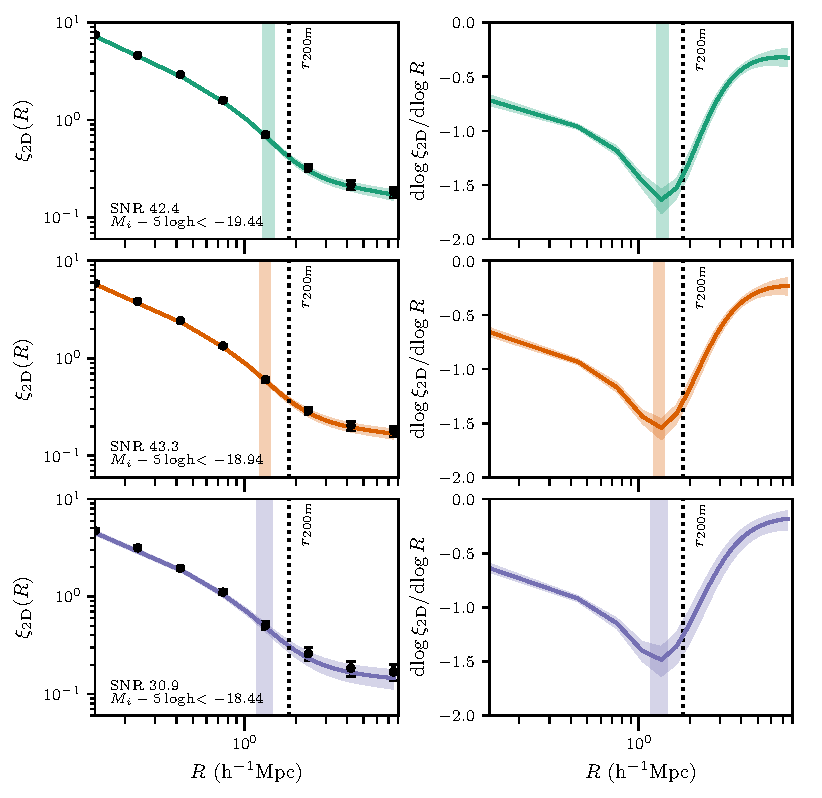
\includegraphics[width= \textwidth]{2D_graphs.pdf}
\caption{\textit{Top row: }The estimates of the surface density profiles including the fitted models. The fitted curves indicate the median as well as the 16\% and 84\% quantiles of the model fits. The survey depth of the galaxy catalog increases from left to right (indicated by mag$_{limit}$) and each panel shows two different estimates of the correlation signal using the DP and LS estimator, respectively. The colored vertical lines indicate the median and 16\% and 84\% quantiles of the location of steepest slope of the profiles as estimated from the minima of the derivatives which are shown in the bottom row. The lightgrey vertical line indicates the location of the R$_{200m}$ radius for comparison. \textit{Bottom row: } The analytical derivatives of the corresponding surface density profiles shown in the top row are displayed. As in the upper panels median, 16\% and 84\% quantiles are given.}
   \label{fig:2D_graphs}
\end{figure*}

\begin{figure*}
    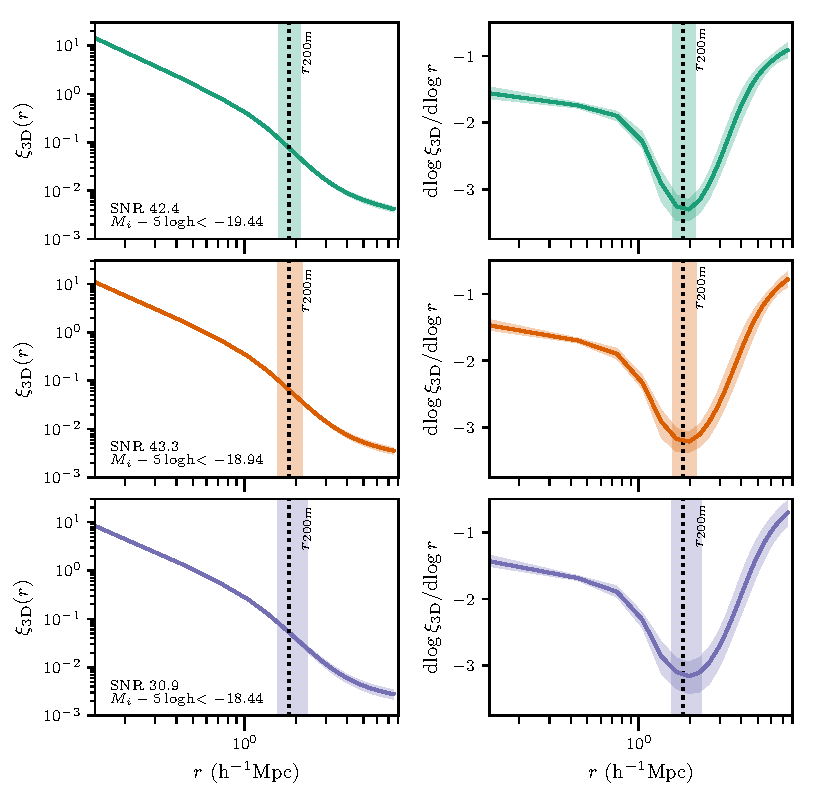
\includegraphics[width= \textwidth]{3D_graphs.pdf}
\caption{\textit{Top row: }The three dimensional density profiles as obtained from the estimates of the fitting parameters obtained through the MCMC procedure. The curves indicate the median (solid lines) as well as the 16\% and 84\% quantiles of the model fit (dashed lines). The survey depth of the galaxy catalog increases from left to right (indicated by mag$_{limit}$) and each panel shows two different estimates of the correlation signal using the DP and LS estimator, respectively. The colored vertical lines indicate the median and 16\% and 84\% quantiles of the location of steepest slope of the profiles as estimated from the minima of the derivatives which are shown in the bottom row. The lightgrey vertical line indicates the location of the R$_{200m}$ radius for comparison. \textit{Bottom row: } The analytical derivatives of the corresponding density profiles shown in the top row are displayed. As in the upper panels median, 16\% and 84\% quantiles are given.}
   \label{fig:3D_graphs} 
\end{figure*}

\begin{figure*}
    \includegraphics[width= \textwidth]{XR_curves.pdf}
\caption{\textit{Top row: }The estimates of the surface density profiles including the fitted models. The fitted curves indicate the median as well as the 16\% and 84\% quantiles of the model fits. The survey depth of the galaxy catalog increases from left to right (indicated by mag$_{limit}$) and each panel shows two different estimates of the correlation signal using the DP and LS estimator, respectively. The colored vertical lines indicate the median and 16\% and 84\% quantiles of the location of steepest slope of the profiles as estimated from the minima of the derivatives which are shown in the bottom row. The lightgrey vertical line indicates the location of the R$_{200m}$ radius for comparison. \textit{Bottom row: } The analytical derivatives of the corresponding surface density profiles shown in the top row are displayed. As in the upper panels median, 16\% and 84\% quantiles are given.}
   \label{fig:XR_graphs}
\end{figure*}

\begin{table*}
    \centering
    \caption{fit parameters (incomplete)}
    \label{tab:fit_parameters}
    \begin{tabular}{|c|c|c|c|c|c|c|c|c|c|c|c|}
    \hline 
    clu & depth & est & $\log_{10}(\rho_s)$ & $\log_{10}(\alpha)$ & $\log_{10}(r_s)$ & $\log_{10}(\rho_0)$ & $s_e$ & $\log_{10}(r_t)$ & $\log_{10}(\beta)$ & $\log_{10}(\gamma)$ & $\chi^2/\nu$ \\ 
    \hline 
    \hline
  PSZ2 & 21 & DP & $-0.48^{+0.30}_{-0.33}$ & $-0.49^{+0.30}_{-0.33}$ & $-0.48^{+0.30}_{-0.33}$ & $-0.48^{+0.30}_{-0.33}$ & $-0.48^{+0.30}_{-0.33}$ & $-0.48^{+0.30}_{-0.33}$ & $-0.48^{+0.30}_{-0.33}$ & $-0.48^{+0.30}_{-0.33}$ & $8.3^{+3.6}_{-2.5}$ \\ 
    \hline 
  PSZ2 & 21 & LS & $-0.48^{+0.30}_{-0.33}$ & $-0.48^{+0.30}_{-0.33}$ & $-0.48^{+0.30}_{-0.33}$ & $-0.48^{+0.30}_{-0.33}$ & $-0.48^{+0.30}_{-0.33}$ & $-0.48^{+0.30}_{-0.33}$ & $-0.48^{+0.30}_{-0.33}$ & $-0.48^{+0.30}_{-0.33}$ & $-0.48^{+0.30}_{-0.33}$ \\ 
    \hline 
   PSZ2 & 21.5 & DP & $-0.48^{+0.30}_{-0.33}$ & $-0.48^{+0.30}_{-0.33}$ & $-0.48^{+0.30}_{-0.33}$ & $-0.48^{+0.30}_{-0.33}$ & $-0.48^{+0.30}_{-0.33}$ & $-0.48^{+0.30}_{-0.33}$ & $-0.48^{+0.30}_{-0.33}$ & $-0.48^{+0.30}_{-0.33}$ & $-0.48^{+0.30}_{-0.33}$ \\
    \hline
   PSZ2 & 21.5 & LS & $-0.48^{+0.30}_{-0.33}$ & $-0.48^{+0.30}_{-0.33}$ & $-0.48^{+0.30}_{-0.33}$ & $-0.48^{+0.30}_{-0.33}$ & $-0.48^{+0.30}_{-0.33}$ & $-0.48^{+0.30}_{-0.33}$ & $-0.48^{+0.30}_{-0.33}$ & $-0.48^{+0.30}_{-0.33}$ & $-0.48^{+0.30}_{-0.33}$ \\
    \hline
   PSZ2 & 22 & DP & $-0.48^{+0.30}_{-0.33}$ & $-0.48^{+0.30}_{-0.33}$ & $-0.48^{+0.30}_{-0.33}$ & $-0.48^{+0.30}_{-0.33}$ & $-0.48^{+0.30}_{-0.33}$ & $-0.48^{+0.30}_{-0.33}$ & $-0.48^{+0.30}_{-0.33}$ & $-0.48^{+0.30}_{-0.33}$ & $-0.48^{+0.30}_{-0.33}$ \\
    \hline
   PSZ2 & 22 & LS & $-0.48^{+0.30}_{-0.33}$ & $-0.48^{+0.30}_{-0.33}$ & $-0.48^{+0.30}_{-0.33}$ & $-0.48^{+0.30}_{-0.33}$ & $-0.48^{+0.30}_{-0.33}$ & $-0.48^{+0.30}_{-0.33}$ & $-0.48^{+0.30}_{-0.33}$ & $-0.48^{+0.30}_{-0.33}$ & $-0.48^{+0.30}_{-0.33}$ \\
    \hline
   MCXC & 21 & DP & $-0.48^{+0.30}_{-0.33}$ & $-0.48^{+0.30}_{-0.33}$ & $-0.48^{+0.30}_{-0.33}$ & $-0.48^{+0.30}_{-0.33}$ & $-0.48^{+0.30}_{-0.33}$ & $-0.48^{+0.30}_{-0.33}$ & $-0.48^{+0.30}_{-0.33}$ & $-0.48^{+0.30}_{-0.33}$ & $-0.48^{+0.30}_{-0.33}$ \\
    \hline
   MCXC & 21.5 & DP & $-0.48^{+0.30}_{-0.33}$ & $-0.48^{+0.30}_{-0.33}$ & $-0.48^{+0.30}_{-0.33}$ & $-0.48^{+0.30}_{-0.33}$ & $-0.48^{+0.30}_{-0.33}$ & $-0.48^{+0.30}_{-0.33}$ & $-0.48^{+0.30}_{-0.33}$ & $-0.48^{+0.30}_{-0.33}$ & $-0.48^{+0.30}_{-0.33}$ \\
    \hline
   MCXC & 22 & DP & $-0.48^{+0.30}_{-0.33}$ & $-0.48^{+0.30}_{-0.33}$ & $-0.48^{+0.30}_{-0.33}$ & $-0.48^{+0.30}_{-0.33}$ & $-0.48^{+0.30}_{-0.33}$ & $-0.48^{+0.30}_{-0.33}$ & $-0.48^{+0.30}_{-0.33}$ & $-0.48^{+0.30}_{-0.33}$ & $-0.48^{+0.30}_{-0.33}$ \\
    \hline
    \end{tabular} 
\end{table*}

\begin{table}
    \centering
    \caption{We list the signal to noise ratios (SNRs) of the different sets of data-points. For comparison: The SNR achieved by \citet{more2016detection} is 263. It is much higher due to size of the cluster sample used in their study.}
    \label{tab:snr}
    \begin{tabular}{|c|c|c|c|c|c|c|c|c|c|}
    \hline
    clu & PSZ2 & PSZ2 & PSZ2 & PSZ2 & PSZ2 & PSZ2 & MCXC & MCXC & MCXC\\  
    \hline 
    depth & 21 & 21 & 21.5 & 21.5 & 22 & 22 & 21 & 21.5 & 22\\ 
    \hline
   est & DP & LS & DP & LS & DP & LS & DP & DP & DP\\ 
    \hline 
   SNR & 23.2 & 16.2 & 20.3 & 16.5 & 17.5 & 13.3 & & &\\ 
    \hline
    \end{tabular} 
\end{table}

\subsection{Location of the Splashback radius}
Using the estimates of the fitting parameters obtained from the MCMC procedure the posterior distributions of the locations of the splashback radii as inferred from the different datasets are obtained. The histograms are shown in Figure~\ref{fig:splashback}, where the panels on the left display the posterior distributions of the projected splashback radius and the right panels the distributions of the three dimensional, physical counterparts. The top row shows the results as inferred by using the DP estimator whereas the LS estimator was used in the lower panels. The survey depth is indicated for each distribution and the used color code corresponds to the code used in Figure~\ref{fig:2D_graphs} and Figure~\ref{fig:3D_graphs}. The inferred medians as well as the 16\% and 84\% quantiles of the distributions are listed in Table~\ref{tab:splashbacks}. 
The choice of the estimator does not influence the location of the splashback radius, as it was already visible from the shapes of the density profiles above. But increasing the survey depth shifts the location to smaller radii. This trend is visible for the two and three dimensional splashback radii. It can also be observed that the constraints on the projected splashback radius are more stringent than on its three dimensional counterparts.


\begin{figure*}
    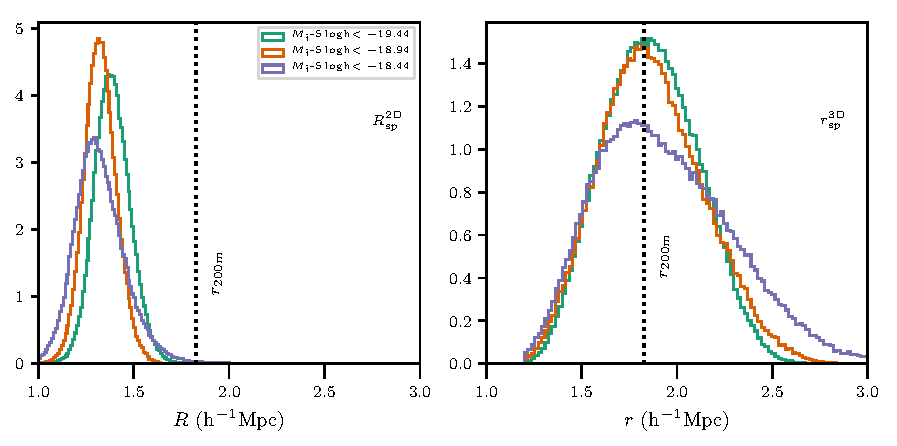
\includegraphics[width= \textwidth]{splashback.pdf}
\caption{Shown are the posterior distributions of the inferred locations of the splashback radii. On the left side the distributions of the projected splashback radii are shown whereas the distributions of the three dimensional counterparts are shown on the right. In the top row the DP estimator is used but the LS estimator is exploited to obtain the distributions in the lower panels. The numbers attached to the distributions indicate the survey depth of the galaxy catalog. Note that the colors of the distributions match with the colors used in Figure~\ref{fig:2D_graphs} and Figure~\ref{fig:3D_graphs}. For reference, the R$_{200m}$ radius is indicated in each panel with a lightgrey, vertical, dashed line.}
   \label{fig:splashback} 
\end{figure*}

\begin{figure*}
    \includegraphics[width= \textwidth]{xr_splashback.pdf}
\caption{Shown are the posterior distributions of the inferred locations of the splashback radii. On the left side the distributions of the projected splashback radii are shown whereas the distributions of the three dimensional counterparts are shown on the right. In the top row the DP estimator is used but the LS estimator is exploited to obtain the distributions in the lower panels. The numbers attached to the distributions indicate the survey depth of the galaxy catalog. Note that the colors of the distributions match with the colors used in Figure~\ref{fig:2D_graphs} and Figure~\ref{fig:3D_graphs}. For reference, the R$_{200m}$ radius is indicated in each panel with a lightgrey, vertical, dashed line.}
   \label{fig:splashback} 
\end{figure*}

\begin{table}
    \centering
    \caption{We list the findings of the splashback radii (incomplete)}
    \label{tab:splashbacks}
    \begin{tabular}{|c|c|c|c|c|c|c|c|c|c|}
    \hline
    clu & PSZ2 & PSZ2 & PSZ2 & PSZ2 & PSZ2 & PSZ2 & MCXC & MCXC & MCXC \\ 
    \hline 
    depth & 21 & 21 & 21.5 & 21.5 & 22 & 22 & 21 & 21.5 & 22\\ 
    \hline
   est & DP & LS & DP & LS & DP & LS & DP & DP & DP\\ 
    \hline 
   R$_{sp}^{2D}$ & LS & & & & & & & &\\ 
    \hline 
   r$_{sp}^{3D}$ & DP & & & & & & & &\\
    \end{tabular} 
\end{table}


\subsection{Deprojection}
In Figure~\ref{fig:deprojection} the estimates of the three dimensional density profiles as obtained from the alternative deprojection algorithm described in Section~\ref{sec:Deprojection} are presented. The deprojection method was exploited for each one of the three galaxy catalogs. The survey depth increases from left to right. The density profiles obtained by the standard MCMC fitting procedure outlined above are added to the data-points for better comparison. One can observe that the data points agree well with the density profiles obtained from the standard procedure on scales below 2 h$^{-1}$ Mpc but possess an overshoot on larger scales.

\begin{figure*}
    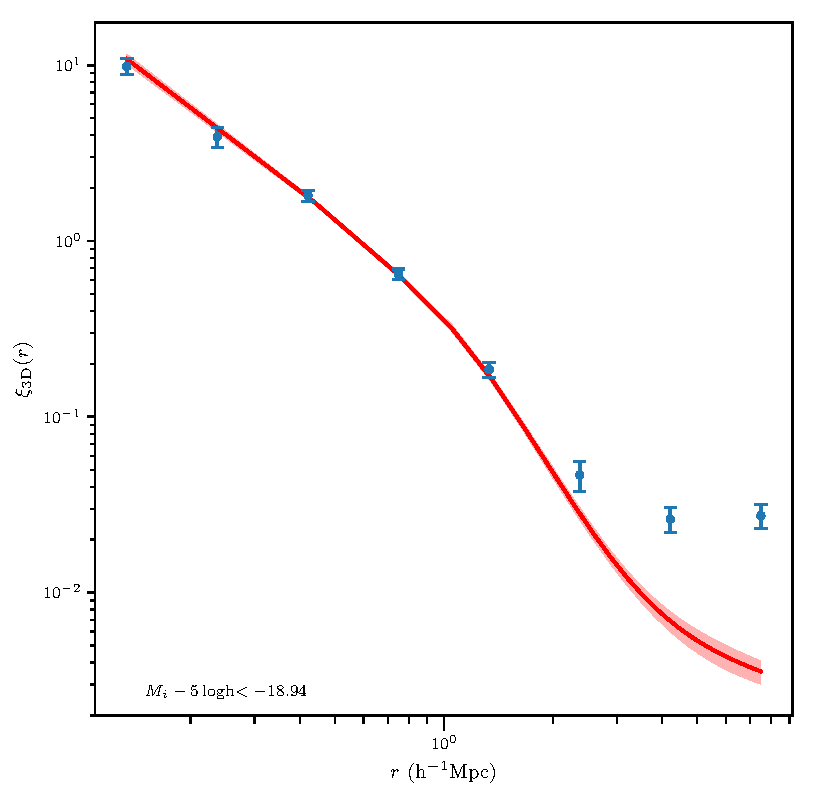
\includegraphics[width= \textwidth]{deprojection.pdf}
\caption{The data-points indicate the estimates of the three dimensional density profiles as inferred by using the deprojection algorithm outlined in Section~\ref{sec:Deprojection}. Additionally, the density profiles as obtained by using the DP estimator and the standard MCMC fitting procedure are shown for comparison. The survey depth increases from left to right and is indicated by mag$_{limit}$.}
   \label{fig:deprojection} 
\end{figure*}




\subsection{Separation of red and blue galaxies (incomplete)}


\section{Discussion (incomplete)}

\subsection{Density profiles}



why are shapes different?
compare with redmapper
as expected? splashback feature visible?

\subsection{Location of the Splashback radius}
show $splash_comp$
show derivatives
why is rsp different for each sample
why different from redmapper
measurements consistent?
measurements consistent with theory?
do max derivatives make sense (reference to paper)

\begin{figure}
    \includegraphics[width= \columnwidth]{splash_comp.pdf}
\caption{bla}
   \label{fig:splash_comp} 
\end{figure}


\subsection{Deprojection}

Do rhos differ? Why?
does deprojection work?
how to imporove?

\subsection{Separation of red and blue galaxies}
why different?
expected result?


\section{Conclusions}

The last numbered section should briefly summarise what has been done, and describe
the final conclusions which the authors draw from their work.

\section*{Acknowledgements}
The Pan-STARRS1 Surveys (PS1) and the PS1 public science archive have been made possible through contributions by the Institute for Astronomy, the University of Hawaii, the Pan-STARRS Project Office, the Max-Planck Society and its participating institutes, the Max Planck Institute for Astronomy, Heidelberg and the Max Planck Institute for Extraterrestrial Physics, Garching, The Johns Hopkins University, Durham University, the University of Edinburgh, the Queen's University Belfast, the Harvard-Smithsonian Center for Astrophysics, the Las Cumbres Observatory Global Telescope Network Incorporated, the National Central University of Taiwan, the Space Telescope Science Institute, the National Aeronautics and Space Administration under Grant No. NNX08AR22G issued through the Planetary Science Division of the NASA Science Mission Directorate, the National Science Foundation Grant No. AST-1238877, the University of Maryland, Eotvos Lorand University (ELTE), the Los Alamos National Laboratory, and the Gordon and Betty Moore Foundation.

Based on observations obtained with Planck (http://www.esa.int/Planck), an ESA science mission with instruments and contributions directly funded by ESA Member States, NASA, and Canada.

Some of the results in this paper have been derived using the HEALPix (K.M. Górski et al., 2005, ApJ, 622, p759) package

\bibliographystyle{mnras}
\bibliography{RSP_library} 

\newpage

\appendix

\section{Additional Figures}
\label{sec:figures}

\begin{figure}
    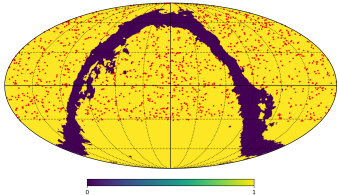
\includegraphics[width= \columnwidth]{Planck_pres.png}
\caption{HEALPix map showing the used cluster positions as selected from the PSZ2 catalog. In total 596 clusters have been selected. The violet area marks the region that is excluded by the survey selection function. Note that all clusters with $\delta<-31\degr$ have been removed since this region is not covered by the Pan-STARRS 3$\upi$ Steradian survey. The ICRS coordinate system is used.}
    \label{fig:planck_fig} 
\end{figure}

\begin{figure*}
    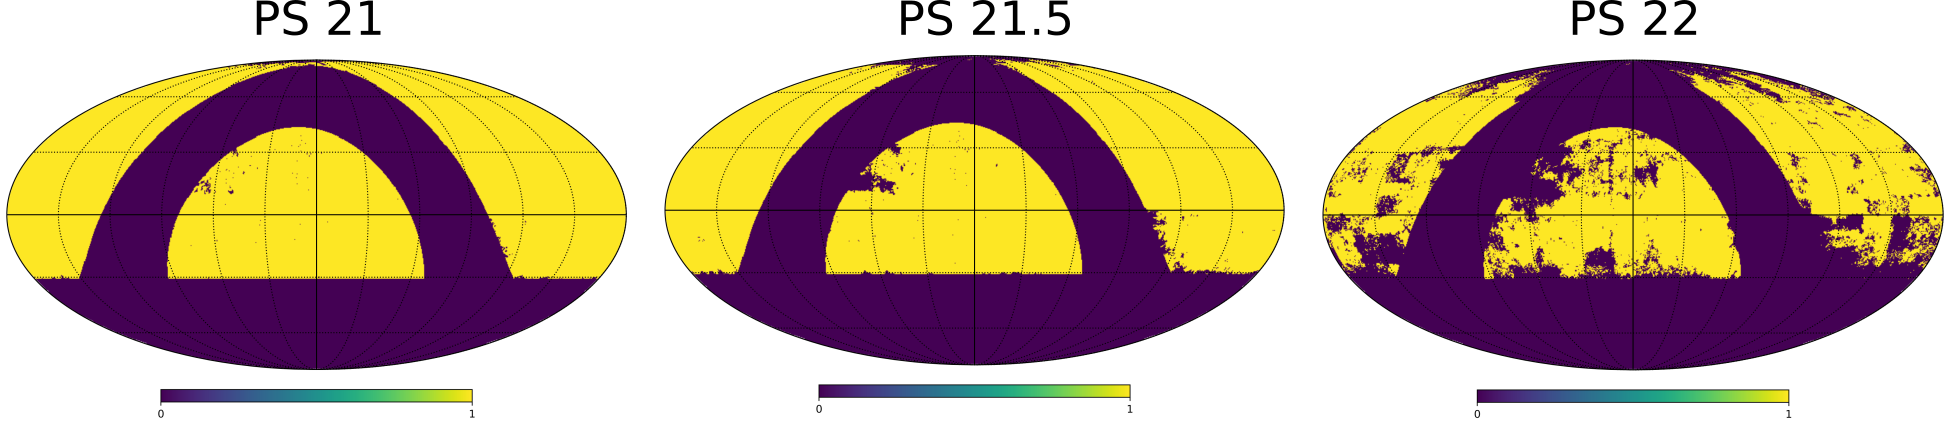
\includegraphics[width= \textwidth]{heal_maps.png}
\caption{HEALPix map showing the disregarded regions of the Pan-STARRS 3$\upi$ Steradian survey in violet. The lower magnitude limit is 21.0, 21.5 and 22.0 respectively and ICRS coordinates are used.}
   \label{fig:heal_map} 
\end{figure*}

\section{Convergence of MCMC chains}
\label{sec:convergence}
Three different methods are exploited in order to assess the convergence of the MCMC chains. Firstly, the general behavior of the chains is monitored and it is checked that they are well behaved, meaning that they converge to a common point in the parameter space, at least visually. With the same goal in mind the autocorrelations of the chains are calculated and it is assured that the autocorrelations are monotonically decreasing as the chains grow.

The second method involves performing a statistical test, named after Geweke \citet{geweke1991evaluating} which relies on methods from spectral analysis to address the issues of biases and variance alike. Imagine attempting to estimate the mean of a function $f$ which depends on the simulated parameter $\theta$. After $n$ iterations of the chain the estimate of the mean becomes
\begin{equation}
\bar{f}_n=\frac{\sum_{i=1}^n f(\theta^{(i)})}{n}
\end{equation}
and Geweke states that the asymptotic variance of that estimator yields $S^G(0)/n$, where $S^G(0)$ indicates the spectral density at frequency 0. The Geweke statistic is calculated by using two subsamples of the simulated parameter set. Geweke suggests taking the first 10\% of the iterations as the first sample $n_A$ and the last 50\% of the iterations to be the second sample $n_B$. Note that $n_A/n + n_B/n < 1$ to assure asymptotic independence of the two parts of the chain. For both subsets the estimate of the mean is calculated yielding $\bar{f}(\theta)_A$ and $\bar{f}(\theta)_B$, respectively. Further, the corresponding asymptotic variances are calculated as well to obtain $S^G_A(0)/n_A$ and $S^G_B(0)/n_B$, respectively. Geweke's convergence diagnostic is than constructed as
\begin{equation}
Z_{(A,B)}=\frac{\bar{f}(\theta)_A-\bar{f}(\theta)_B}{n_A^{-1}S^G_A(0)-n_B^{-1}S^G_B(0)},
\end{equation}
which approaches a standard normal distribution according to the central limit theorem if the samples are being drawn from a stationary distribution. Geweke argues that the convergence statistic may be used to determine how many of the initial steps must be regarded as burn-in steps and therefore must be disregarded \citet{cowles1996markov}.

Lastly, the Heidelberger and Welch test is performed \citep{heidelberger1983simulation}. The test combines approaches from spectral analysis with a convergence test by \citet{schruben1983optimal} designed to detect non-stationarity in a simulated set of parameters. Denoting the jth simulated parameter value in the chain as $\theta_j$ and the total number of iterations in the chain as $n$ the statistic $B_n(t)$ is calculated as
\begin{equation}
B_n(t)=\frac{T_{[nt]}-[nt]\bar{\theta}}{\sqrt{nS(0)}} , 0 \leq t \leq 1
\end{equation}
where $[.]$ indicates the floor function and
\begin{align}
T_k=\sum_{j=1}^k \theta_j \\
\bar{\theta}=\frac{\sum_{j=1}^n \theta_j}{n}
\end{align}
and $S(0)$ indicates the spectral density at frequency 0 once again. The claim is that if convergence of the chain is given, meaning that a stationary distribution is reached the statistic $B_n(t)$ is approximately distributed as a Browninan bridge. The Cramer-von Mises statistic 
\begin{equation}
\int_0^1 B_n(t)^2 dt
\end{equation}
may than be used as a test statistic to test if $B_n(t)$ tracks a Brownian bridge and therefore to test the hypothesis of convergence of the underlying chain \citep{cowles1996markov}.

Note that, as highlighted by \citet{cowles1996markov}, there exists no universally reliable tool to assure the convergence of a MCMC chain. Instead, it is advisable to use a variety of different tools that are aimed at doing so. Therefore, even though the chains seem to converge according to the statistical tests exploited, the tests may fail and the chains did not converge after all \citep{cowles1996markov}.

The statistical tests mentioned above have been carried out using the \fnurl{py-coda}{https://github.com/surhudm/py-coda} package which provides a python wrapper of some of the tools included in the CODA package in R \citep{coda}. 
\section{Deprojection of the surface density profile}
\label{sec:deprojection_math}
We follow the procedure outlined by \citet{eisenstein2003deprojecting} to construct an estimator which can recover the spatial density profile from the observed surface density profile. The projected angular galaxy distribution $\Sigma(R)$ of a cluster can be found from the spatial distribution $\rho(r)$ by integration along the line of sight as
\begin{equation}
\Sigma(R)=\int_{-\infty}^{\infty} \rho(\sqrt{R^2+Z^2})dZ. \label{eq:c1}
\end{equation}
It is known that the integral in Equation~\ref{eq:c1} can be inverted as an Abel integral to obtain
\begin{equation}
\rho(r) = -\frac{1}{\pi} \int_{r}^{\infty} \frac{d\Sigma}{dR}\frac{dR}{\sqrt{R^2-r^2}}. \label{eq:c2}
\end{equation}
Involving a derivative of the measured quantity $\Sigma(R)$ this integral is very noisy and therefore difficult to compute in practice. To overcome this we consider measuring $\Sigma(R)$ only as an integral weighted by as window function $W(r)$, where the choice of $W(r)$ can be used to pick up the number of galaxies in a radial bin. Therefore, $\Sigma(R)$ is approximated by the galaxy count $\Delta$ as  
\begin{equation}
\Delta N = \int_{0}^{\infty} W(r) \rho(r) 4 \pi r^2 dr.
\end{equation}
We proceed by using Equation~\ref{eq:c2} and partial integration as
\begin{align}
\Delta N &=& \int_{0}^{\infty} W(r) \left[ \frac{-1}{\pi} \int_{r}^{\infty} \frac{d\Sigma}{dR}\frac{dR}{\sqrt{R^2-r^2}} \right] 4 \pi r^2 dr  \label{eq:rho} \\
&=& -\frac{1}{\pi} \int_{0}^{\infty} dR \frac{d\Sigma}{dR} \int_{0}^{R} 4 \pi r^2 W(r) \frac{dr}{\sqrt{R^2-r^2}}\\
&=& -4 \int_{0}^{\infty} dR \frac{d\Sigma}{dR} \int_{0}^{R} W(r) \frac{r^2 dr}{\sqrt{R^2-r^2}} \\
&=& -4 \int_{0}^{\infty} dR \frac{d\Sigma}{dR} G(R)\\
&=& 4 \int_{0}^{\infty} dR \frac{dG}{dR} \Sigma(R) \label{eq:parts}\\
&=& 4 \int_{0}^{\infty} dR \frac{dG}{dR} \sum_i \frac{\delta_{\rm D}(R-R_i)}{2\pi R_i} \label{eq:discrete} \\
&=& \sum \frac{2}{\pi R_i} \left.\frac{dG}{dR}\right|_{R_i}
\end{align}
where we replaced the angular distribution by a discrete sum over the single galaxies in the sample located at projected radii $R_i$ from the cluster center and we defined
\begin{equation}
G(R) = \int_{0}^{R} W(r) \frac{r^2 dr}{\sqrt{R^2-r^2}}.
\end{equation}
Let us parametrize the three dimensional distance as $r=R \sin(\theta)$ yielding
\begin{align}
G(R) &=& \int_{0}^{\pi/2} W(R\sin\theta) \frac{R^2 \sin^2\theta R \cos\theta d\theta}{R\cos\theta}\\
&=& \int_{0}^{\pi/2} W(R\sin\theta) R^2 \sin^2\theta  d\theta.
\end{align}
Now let us consider a radial bin $r\in[a, b]$, thus $W(r)=\Theta(r-a) - \Theta(r-b)$, where $\Theta$ is the Heaviside step function. In this case we have three regimes for any given radius $R$; (i) $R<a$, (ii) $R\in[a, b]$, (iii) $R>b$. Let us deal with each of these cases separately.

\paragraph{Case (i): $R<a$}
In case (i), $\forall \theta\in[0, \pi/2]$, $W(R\sin\theta)=0$. Therefore, $G(R)=0$ and hence the derivative is zero.

\paragraph{Case (ii): $R\in[a,b]$}
In case (ii), $W(R\sin\theta)$ is non-zero $\forall \theta\in[\theta_{\rm min}, \pi/2]$, where $R\sin\theta_{\rm min}=a$. Therefore, the integral for G(R) reduces to
\begin{eqnarray}
G(R) &=& \int_{\theta_{\rm min}}^{\pi/2} R^2 \sin^2\theta  d\theta \\
&=& \frac{R^2}{2} \left[\theta-\sin\theta\cos\theta\right]_{\theta_{\rm min}}^{\pi/2}\\
&=& \frac{R^2}{2} \left[ \frac{\pi}{2} - (\theta_{\rm min}-\sin\theta_{\rm min}\cos\theta_{\rm min})  \right] \\
\frac{dG}{dR} &=& R  \frac{\pi}{2} -  R  \left[\tan^{-1}\left(\frac{x/R}{\sqrt{1-x^2/R^2}}\right) - \frac{x/R}{\sqrt{1-x^2/R^2}}\right]_a \nonumber \\
&=& R \left[ \frac{\pi}{2} - f(a) \right] \\
\frac{2}{\pi R}\frac{dG}{dR} &=& 1 - \frac{2}{\pi} f(a)
\end{eqnarray}
where we defined
\begin{equation}
f(x)=\tan^{-1}\left(\frac{x/R}{\sqrt{1-x^2/R^2}}\right) - \frac{x/R}{\sqrt{1-x^2/R^2}}
\end{equation}

\paragraph{Case (iii): $R>b$}
In case (iii), $W(R\sin\theta)$ is non-zero $\forall \theta\in[\theta_{\rm min}, \theta_{\rm max}]$, where $R\sin\theta_{\rm min}=a$, and $R\sin\theta_{\rm max}=b$. Therefore, the integral for G(R) reduces to
\begin{eqnarray}
G(R) &=& \int_{\theta_{\rm min}}^{\theta_{\rm max}} R^2 \sin^2\theta  d\theta \\
&=& \frac{R^2}{2} \left[\theta-\sin\theta\cos\theta\right]_{\theta_{\rm min}}^{\theta_{\rm max}}\\
&=& \frac{R^2}{2} \left[\sin^{-1}\left(\frac{x}{R}\right) - \frac{x}{R}\sqrt{1-\frac{x^2}{R^2}} \right]_{a}^{b} \\
&=& \left[\frac{R^2}{2} \sin^{-1}\left(\frac{x}{R}\right) - \frac{x}{2}\sqrt{R^2-x^2} \right]_{a}^{b} \\
\frac{dG}{dR} &=& \left[R  \sin^{-1}\left(\frac{x}{R}\right) - \frac{1}{2} \frac{x}{\sqrt{1-x^2/R^2}} - \frac{x}{2}\frac{1}{\sqrt{1-x^2/R^2}}\right]_a^b\\
\frac{dG}{dR} &=& R  \left[\sin^{-1}\left(\frac{x}{R}\right) - \frac{x/R}{\sqrt{1-x^2/R^2}}\right]_a^b\\
\frac{dG}{dR} &=& R  \left[\tan^{-1}\left(\frac{x/R}{\sqrt{1-x^2/R^2}}\right) - \frac{x/R}{\sqrt{1-x^2/R^2}}\right]_a^b \\
&=& R [f(b) - f(a)] \\
\frac{2}{\pi R}\frac{dG}{dR} &=& \frac{2}{\pi} [ f(b) - f(a)]
\end{eqnarray}

\subsection{Masking and survey boundaries}
The surface area normalization in Eq.~\ref{eq:discrete} assumes that the entire annulus at radius $R_i$ around a given cluster lays within the survey area. But this may not be true due to masking effects or survey boundaries. In this case the normalization is modified to be
\begin{equation}
\Sigma(R) = \sum_i \frac{1}{2\pi\phi(R)} \delta_{\rm D}(R-R_i),
\end{equation}
where $\phi(R)$ is the fraction of the annulus that lays within the survey area.


\bsp
\label{lastpage}
\end{document}
